%!TEX root = main_zh.tex
\section{背景与动机}
\label{sec:background}

\subsection{LLM 调度问题}
\label{subsec:problem}

\phm{LLM 推理负载的需求\emph{不确定性}与\emph{混合性}。}
大语言模型（LLM）~\cite{deepseek, llama_official}已广泛应用于聊天对话~\cite{openai_chatgpt}、代码生成~\cite{cursor_ai}与具身智能~\cite{wang2023voyager}等场景。
值得注意的是，LLM 推理采用自回归方式：给定输入提示词后，任务会基于当前序列持续生成新 token，直到输出特殊的 \texttt{<EOS>} 标记为止~\cite{yu2022orca}。
如图~\ref{fig:background_uncertainty} 所示，即便提示词固定，\footnote{本文所有推理均使用 0.6 温度，该设置也是许多主流 LLM 的默认值~\cite{llama3_1_8b_instruct,qwen3_32b}。}
不同运行仍会产生不同输出。
因此，请求最终输出长度只能在推理完成后得知，具有显著\emph{不确定性}。

除不确定性外，需求\emph{混合性}也是 LLM 推理的典型特征。
具体而言，推理过程中请求会在 GPU 显存中缓存 token 序列（即 KVCache~\cite{qin2024mooncake}）以避免重复计算；在 vLLM~\cite{vllm_v0_8_2} 等主流框架中，分配 KVCache 是请求能够推进的前提。
图~\ref{fig:background_hybridity} 给出了三个代表性数据集（与~\cite{hu2024inference}一致）上各请求的显存占用与执行时间分布：\emph{SharedGPT}~\cite{sharegpt_vicuna_unfiltered_2025}、\emph{Alpaca-Summarization}~\cite{alpaca_pubmed_summarization_2025}、\emph{Document-Write}~\cite{write_doc_sft_v1_2025}。
结果表明，LLM 服务同时受\emph{计算}与\emph{显存}影响；而传统 OS 工作负载通常主要依据计算代价调度~\cite{cpu_scheduling_comparison_gfg_2026}。

\begin{figure}[t]
    \centering
    \subfigure[从 SharedGPT 中随机采样 10 个提示词，每个提示词重复推理 100 次后的输出长度波动。]{
        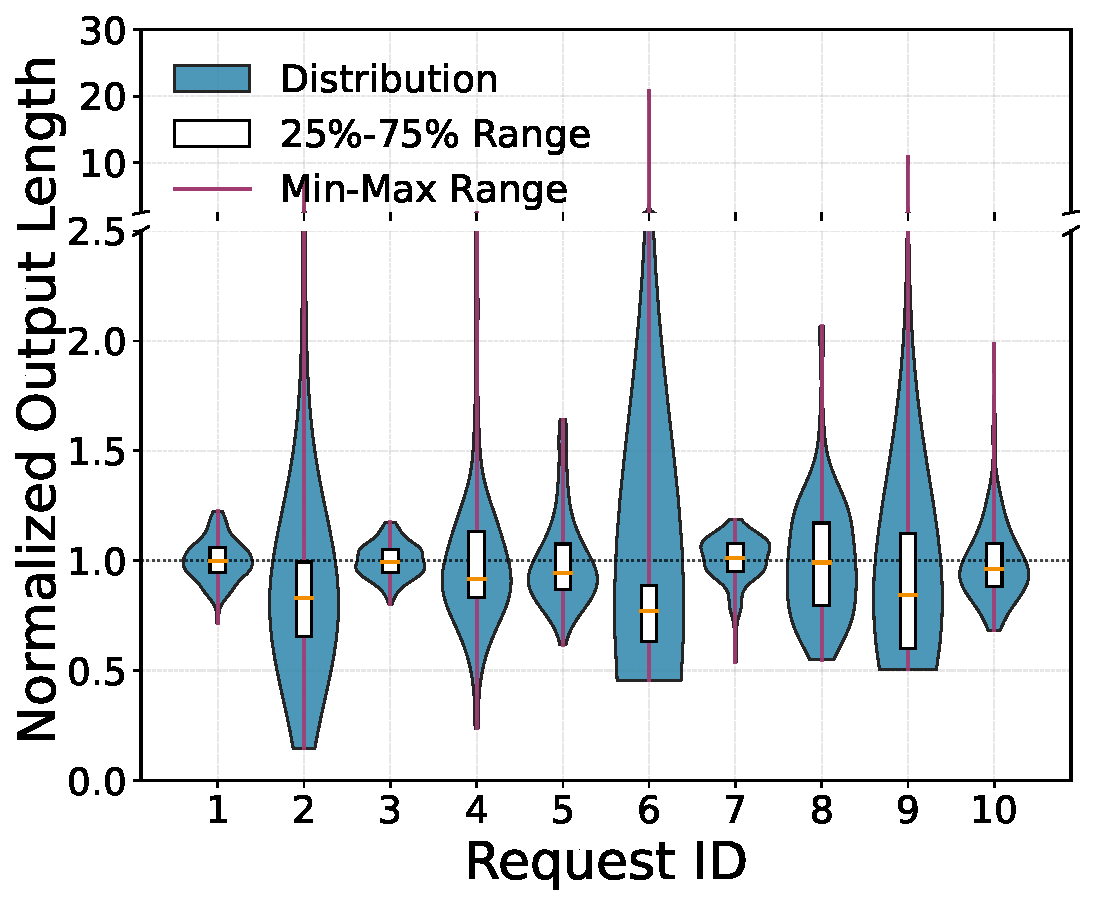
\includegraphics[width=0.45\linewidth]{figures/length_variation.pdf}
        \label{fig:background_uncertainty}
    }
    \hfill
    \subfigure[三个数据集请求在 H800 GPU 上单独剖析得到的散点图（执行时间，峰值显存占用）。]{
        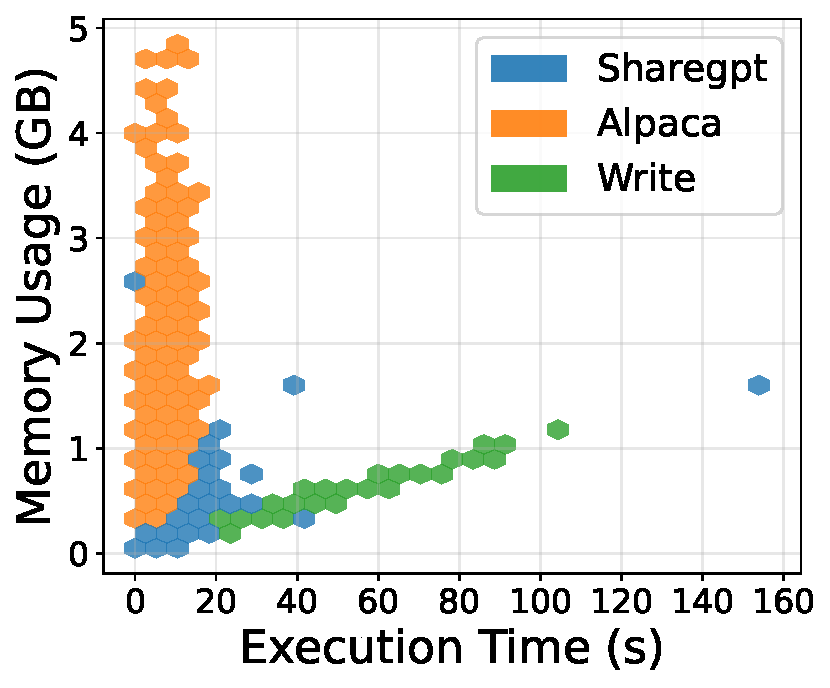
\includegraphics[width=0.45\linewidth]{figures/demand_hybridity.pdf}
        \label{fig:background_hybridity}
    }
    \caption{LLM 推理资源需求\emph{不确定性}与\emph{混合性}的实证证据。}
    \label{fig:background_uncertainty_and_hybridity}
\end{figure}

\phm{调度是 LLM 后端性能的关键。}
随着 LLM 需求爆发，来自不同用户的请求常在共享后端中处理，不同请求会竞争有限的计算与显存资源~\cite{Recasens2025Mind}。
为了提升用户体验，必须通过合理调度降低整体延迟。
尽管 LLM 有多种时延指标（TTFT、TPOT、TTLT），本文以 TTLT 为主，原因在于其综合性\footnote{
第一，TTLT 在智能体等场景中尤为关键：例如 LLM 驱动的机器人控制~\cite{chen2023typefly,wang2024llm}，下游动作通常要等到完整输出后才能启动。
第二，优化 TTLT 往往也会带来其他指标收益。
对于 TTFT，减少队首阻塞通常可直接改善首 token 时延（后续实验也将验证）；
对于 TPOT（统计中常定义为 TTLT 除以输出长度~\cite{wu2023fast,fu2024efficient}），降低 TTLT 也会带来比例改进。
}，这也与多项已有研究保持一致~\cite{shahout2024don,qiu2024efficient}。

\subsection{现有 LLM 调度器的局限}
\label{subsec:limitations}

现有文献已提出多种面向 LLM 推理的调度器。
针对需求不确定性，早期方法多为\emph{与需求无关}的启发式调度。
vLLM~\cite{kwon2023efficient}与 SGLang~\cite{zheng2024sglang}采用 FCFS，易受队首阻塞影响。
为缓解这一问题，FastServe~\cite{wu2023fast}使用\emph{多级反馈队列}（MLFQ），按固定服务配额周期性降低在途请求优先级，本质上近似 \emph{SRPT}，但会引入额外抢占开销。

发现上述不足后，近期调度器开始采用\emph{预测驱动}范式。
例如，SSJF~\cite{qiu2024efficient}利用微调 BERT-base 根据提示词预测输出长度，从而近似 SJF。
同时，Fu 等人~\cite{fu2024efficient}使用 OPT-125M 预测请求输出长度\emph{相对排序}而非绝对值。
近期 TRAIL~\cite{shahout2024don}则用 MLP 在迭代粒度持续预测输出长度，输入为特定 LLM 层特征嵌入。

\begin{figure}[t]
    \centering
    \subfigure[仅预测单一（分桶）值无法覆盖全部输出长度可能性；每个桶对应 100 token 区间。]{
        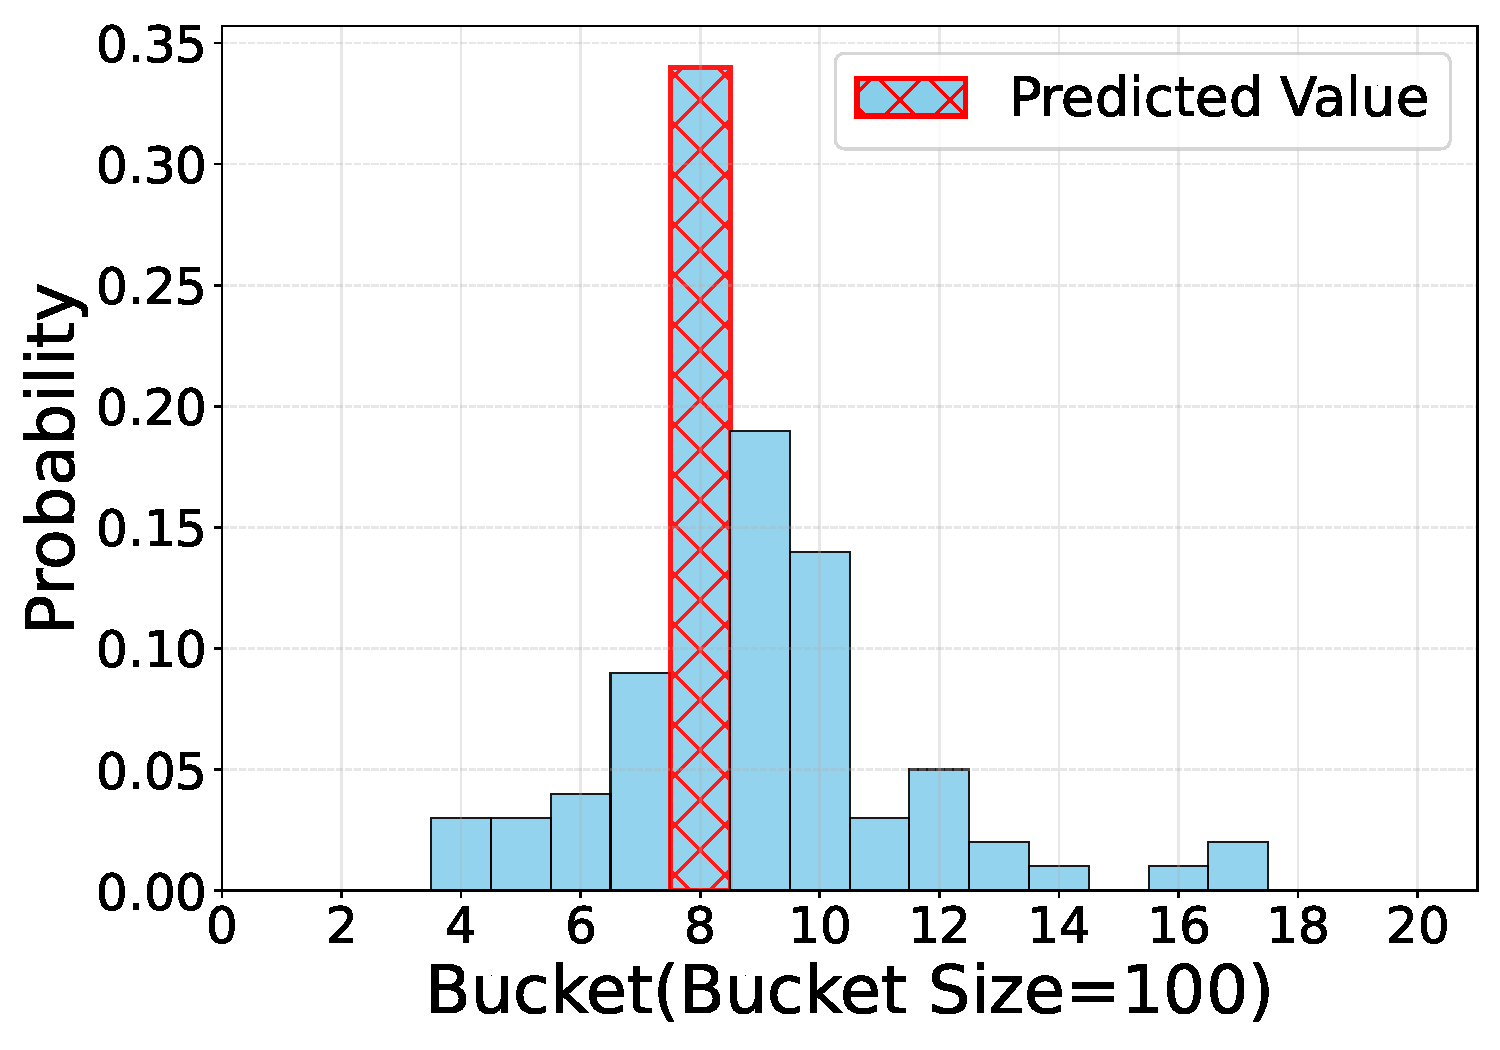
\includegraphics[width=0.53\linewidth]{figures/motivation_low_accuracy.pdf}
        \label{fig:low_prediction_accuracy}
    }
    \hfill
    \subfigure[受 KVCache 约束影响，仅优先短输出请求可能并非最优。]{
        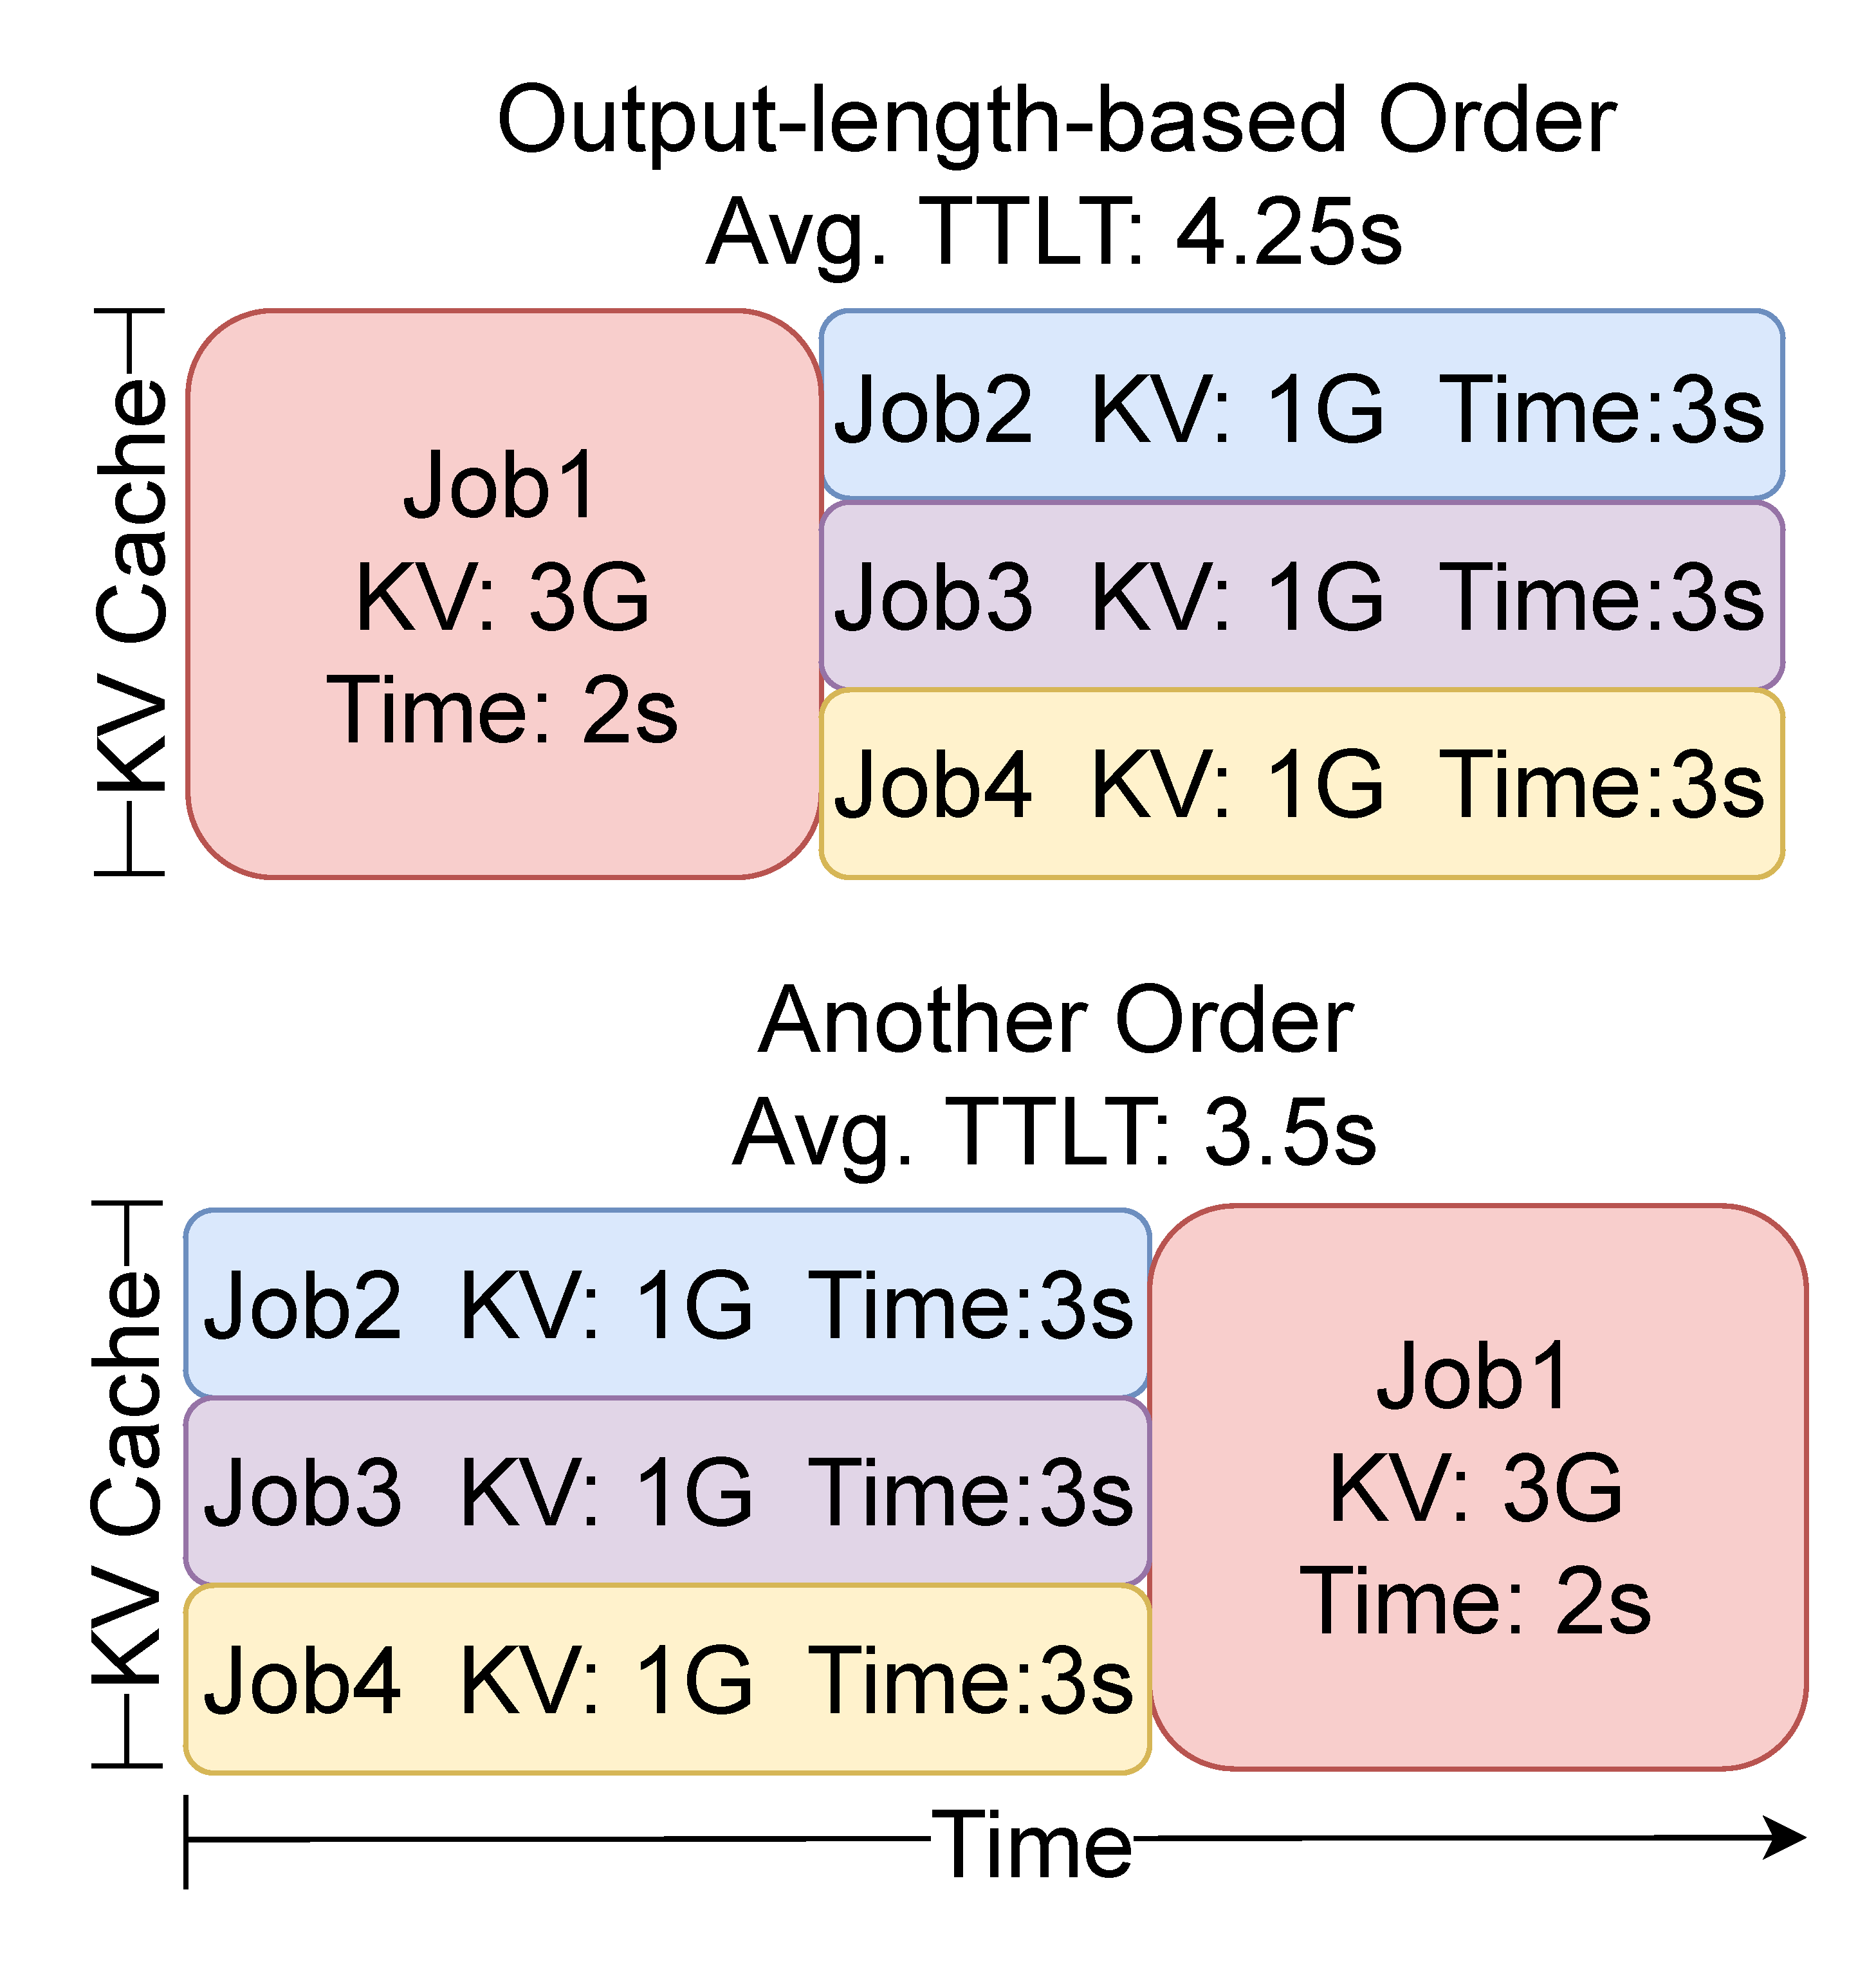
\includegraphics[width=0.37\linewidth]{figures/suboptimality_SJF.pdf}
        \label{fig:wrong_scheduling_order}
    }
    \caption{现有调度器在应对需求不确定性与混合性时的典型缺陷示例。}
    \label{fig:deficiencies}
\end{figure}

但上述预测型调度器在处理\emph{不确定性}方面仍不充分。
第一，它们的长度预测器通常需要较重的离线训练（微调常需 1 万+样本~\cite{jin2023s, fu2024efficient}），且在一个 LLM 上训练的模型难以直接迁移到另一个 LLM。
第二，这些预测器只输出\emph{单一值}，丢失了宝贵的分布信息。
实际上，不确定性是 LLM 推理的内生属性，单值预测很难准确。
如图~\ref{fig:low_prediction_accuracy} 所示，按~\cite{qiu2024efficient}方式使用 DistillBert 进行单值预测时，准确率仅 34.1\%（在 20 个桶中仅命中 1 个）。
而我们在第~\ref{subsec:gittins} 节将展示：保留长度分布信息可带来更优调度决策。
因此，在应对需求不确定性时，应设计一种\emph{免训练}且可直接预测输出长度\emph{分布}的方法。

同时，这些方法在处理需求\emph{混合性}方面也存在不足。
它们通常仅把计算时间（即输出 token 长度）作为服务代价，忽略了 GPU 显存占用。
事实上，输入和输出 token 都会占用 KVCache，因此即便输出长度相同，不同请求的显存代价也可能显著不同。
如图~\ref{fig:wrong_scheduling_order} 所示，当后端受显存瓶颈约束时，仅按“输出更短优先”排序可能是次优的。
因此，要处理 LLM 推理的混合性，必须联合考虑计算与显存两个维度。

综上，受需求不确定性与混合性影响，现有 LLM 调度器难以获得高整体效率。
下一节我们将提出新的高效调度器，分别从输出长度预测、代价建模与请求排队三方面进行优化。
